\documentclass[a4paper]{llncs}
\usepackage[margin=1.5cm]{geometry}
%\usepackage{fullpage}[1in]
%\usepackage{palatino}

\usepackage{makeidx}
\usepackage{amsmath}   
\usepackage[retainorgcmds]{IEEEtrantools}
\usepackage{thumbpdf}
\usepackage{multicol}   
\usepackage{graphicx}   
\usepackage{listings}
\usepackage{algorithm}
\usepackage{algorithmic}
\usepackage{tikz}
\usepackage{subfigure}

\usepackage[
  pagebackref,
  pdfpagelabels,
  extension=pdf,
]{hyperref}
\hypersetup{ 
  pdftitle          = {Learning in a Small World},
  pdfsubject        = {Learning in a Small World},
  pdfauthor         = {Arun Tejasvi Chaganty, Prateek Gaur},
  pdfkeywords       = {},
  pdfcreator        = {pdflatex},
  pdfproducer       = {LaTeX with hyperref and thumbpdf},
  pdfstartpage      = {1},
  pdfpagemode       = UseThumbs,
  colorlinks        = true,
  linkcolor         = red,
  anchorcolor       = red,
  citecolor         = blue,
  filecolor         = red,
  urlcolor          = red
}

% Section References
\newcommand{\secref}[1] {\hyperref[#1]{Section~\ref*{#1}}}
\newcommand{\appendixref}[1] {\hyperref[#1]{Appendix~\ref*{#1}}}
\newcommand{\eqnref}[1] {Equation \eqref{#1}}
\newcommand{\thmref}[1] {Theorem \ref{#1}}
\newcommand{\lmref}[1] {Lemma \ref{#1}}
\newcommand{\algoref}[1] {\hyperref[#1]{Algorithm~\ref*{#1}}}
\renewcommand{\algorithmiccomment}[1]{\textit{// #1}}
%\theoremstyle{plain} \newtheorem{thm}{Theorem}

%Math Operators
\DeclareMathOperator {\argmax} {argmax}
\DeclareMathOperator {\argmin} {argmin}
\DeclareMathOperator {\sgn} {sgn}
\DeclareMathOperator {\trace} {tr}
\DeclareMathOperator{\E} {E}
\DeclareMathOperator{\Var} {Var}

\renewcommand{\Re} {\mathbb{R}}

\newcommand{\ud}{\, \mathrm{d}}
\newcommand{\diff}[1] {\frac{\partial}{\, \partial #1}}
\newcommand{\diffn}[2] {\frac{\partial^{#2}}{\, \partial {#1}^{#2}}}
\newcommand{\tuple}[1] {\langle #1 \rangle}

%Short hand
\newcommand{\states} {\mathcal{S}}
\newcommand{\actions} {\mathcal{A}}
\newcommand{\rewards} {\mathcal{R}}
\newcommand{\graph} {\mathcal{G}}
\newcommand{\mdp} {\mathcal{M}}
\newcommand{\policy} {\pi}
\newcommand{\initset} {\mathcal{I}}
\newcommand{\stopcond} {\beta}
\newcommand{\option} {\tuple{ \initset,\policy,\stopcond} }
\newcommand{\options} {\mathcal{O}}

%Math Operators
\DeclareMathOperator {\Qf} {Q}
\DeclareMathOperator {\Vf} {V}
\newcommand{\epsilonm} {\bar{\epsilon}}


%Math Operators
\DeclareMathOperator {\ball} {B}
\DeclareMathOperator {\ballf} {B^{f}}
\DeclareMathOperator {\sball} {b}
\DeclareMathOperator {\sballf} {b^{f}}

%Short hand
\newcommand{\arbcnst} {\tilde{c}}
\newcommand{\greedyalgo} {\ensuremath{\mathcal{GA}~}}
\newcommand{\egreedyalgo} {\ensuremath{\mathcal{GA}_{\epsilon}~}}


\title{Learning in a Small World}
\author{ Arun Tejasvi Chaganty \and Prateek Gaur \and Ravindran Balaraman \inst{1} } 
\institute{ Department of Computer Science and Engineering, \\
            IIT Madras, Chennai, India - 600036 }

\pagestyle{headings}  % switches on printing of running heads

\frontmatter
\mainmatter

\begin{document}

\maketitle
%\pagebreak

% Outline
\section{Introduction}
\label{sec:intro}

% Problem solving in AI - Why RL
Reinforcement learning (RL) is a widely studied learning framework for
autonomous agents, particularly because of it's extreme generality; it
addresses the problem of learning optimal agent behaviour in an unknown
stochastic environment.

Reinforcement learning (RL) addresses to problem of learning an optimal
behavioural strategy by directly interacting with the environment. 

% Scaling up - challenges - need structure
When scaling up to larger domains, 

% Options as a framework

% What is a useful option - why small world

% Summary of contributions

% General Introduction
In large domains, RL agents generally require a large number of samples to learn
a good policy. The options framework proposed by Sutton, Precup and Singh
\cite{SuttonPrecupSingh1998} provides extended actions for which a policy is
already learnt, reducing the complexity of the learning task, and generally
making the learning task faster. An open question in the options framework is
discovering the options themselves. There has been substantial work to learn
options, mainly focussed around identifying ``bottleneck'' states, either
empirically as in the work bye Stolle \cite{Stolle}, or more recently, using
graph theoretic methods like betweeness \cite{Simsek} or graph partitions
\cite{Simsek2005} explored by Simsek and Barto.

% Motivation
In this work, we propose a method for creating options motivated from a
cognitive perspective, based on the following hypothesis: we memorise many
actions, not necessarily bottleneck ones, and evolve them. Based on their
necessity in solving problems these actions are either reinforced, or gradually
forgotten. The actions could be of varying complexity, and it is intuitive to
expect that we probably learn a great deal more {\em simple} actions than
complex ones. In context of the options framework, these actions correspond to
options, and ``complex actions'' correspond to longer options.

% Our options
A desirable set of options gives the agent a set of skills which can be put
together to efficiently accomplish almost any task. From the perspective of the
state-space interaction graph, this is similar to the problem of distributed
search studied by Kleinberg \cite{Kleinberg}; adding edges to a graph such that
any node can be efficiently reached. Guided by this intuition, the method we
propose generates options using a generalisation of the inverse-square law,
along the lines of the small-world graph generation model proposed by Kleinberg.

% Summary of the results
Our results show that agents trained using our `small-world' options indeed
perform well, and converge to optimal performance quickly and with little
variance. 


\section{Small World Options}
\label{sec:theory}

% What are small world options
In Kleinberg's small-world network model, each node $u$ is given one
`long-range' edge to a node $v$, which was chosen with a probability
$P_r(u,v) \propto \|u-v\|^{-r}$, where $\|u-v\|$ denotes the distance
between $u$ and $v$ in the graph. Similarly for each state $s$, we add
a single `path option' to another state $s'$, where $s'$ is chosen with
probability $P_r(s,s') \propto \|s-s'\|^{-r}$. A path option $o_p(s,s')$
is an option with $\initset = \{s\}$, $\stopcond = \{s'\}$, and an
optimal policy to reach $s'$ for $\pi$. Intuitively, it is an option
that takes the agent from $s$ to $s'$. In practice, we may generate path
options only for a subset of $|S|$. Note that while $O(|S|)$ options are
created, only one additional option is available in any state, and thus
the decision-space for the agent is not significantly larger.

% What is the guarantee we give about them?
On an $r$-dimensional lattice, $\klein_r$, the distance from any node
$u$ to a target node $t$ is bounded by $\|u-t\|$, a quantity which is
locally computable. When given long-range edges distributed according to
$P_r$, Kleinberg showed that the greedy distributed algorithm
$\greedyalgo$ that chooses a neighbour $v$ closest to $t$ will reach $t$
with an expected time $O(\log(|V|)^2)$. This follows as a trivial
corollary of the following theorem,

\begin{theorem}
    \label{thm:small-world}
    %
    Let $f : V \to \Re$ be a function embedded on the graph
    $\graph(V,E)$, such that, $\kappa_1 \|u-v\| - c_1 \le \|f(u)
    - f(v)\| \le \kappa_2 \|u - v\| - c_2$, where $0 \le \kappa_1 \le
    \kappa_2$, and $0 \le c_2 \le \frac{c_1}{2}$. Let $M_f$ be the
    global maxima of $f$. Let \egreedyalgo be an $\epsilon$-greedy
    algorithm with respect to $f$, i.e.  an algorithm which chooses with
    probability $1-\epsilon$ to transit to the neighbouring state
    closest to $M_f$, i.e. $N(u) = \argmin_v \|f(v) - f(M_f)\|$.
    
    If $\graph(V,E)$ is $r$-dimensional lattice, and contains a long
    distance edge distributed $P_r$, then \egreedyalgo takes $O( (\log
    |V|)^2 )$ steps to reach $M_f$.
\end{theorem}
\begin{proof}
  The key insight of the proof is that with edges distributed according
  to $P_r$, there will always be edge within the neighbourhood of a node
  to an exponentially smaller neighbourhood of the target. Thus, the
  agent will only require to hop through $\log |V|$ `neighbourhoods'. By
  bounding the time spent in each neighbourhood to $\log |V|$, we arrive
  at the result. We refer the reader to
  \appendixref{sec:small-world-theory} for the complete proof.
\end{proof}

\begin{figure}[th]
    \centering
    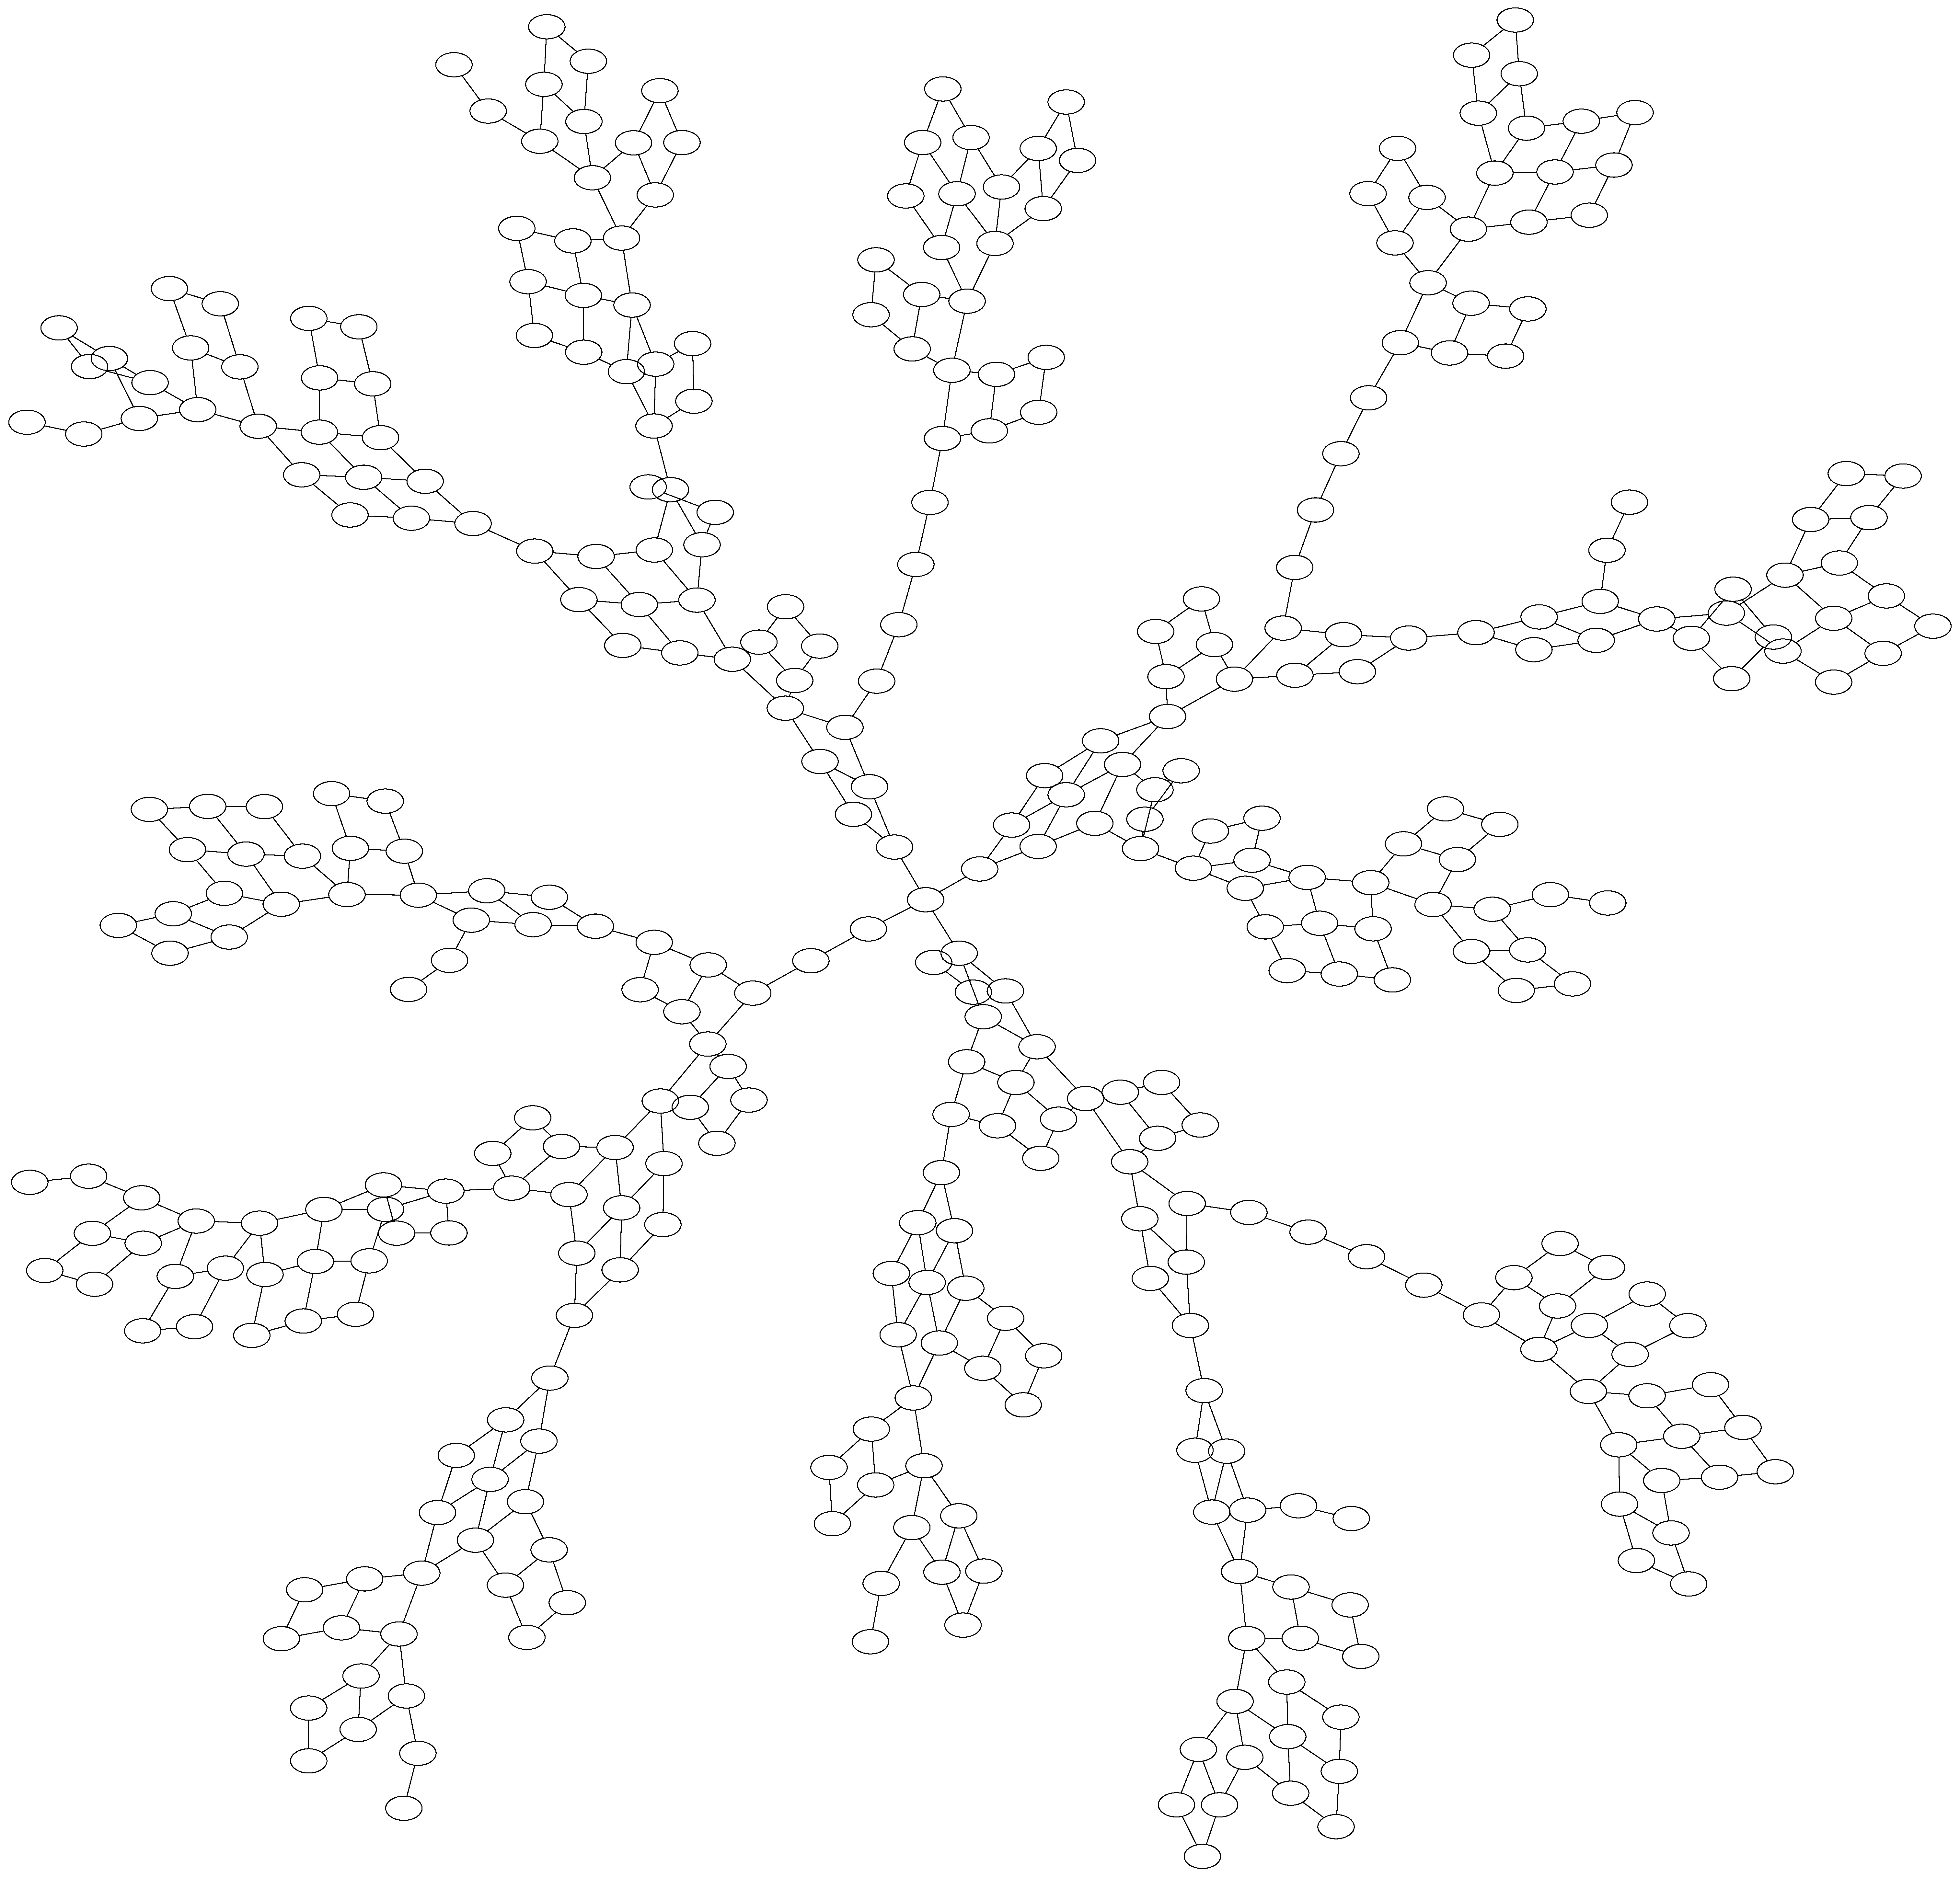
\includegraphics[height=2in]{figures/taxi1}
    \label{fig:taxi-graph}
    \caption{The State Space Graph for Taxi}
\end{figure}

% Graph-based
It is easy to construct a graph $\graph_{\mdp}$ out of the state-space
described by an MDP. The states $\states$ become the nodes of the graph,
and actions $\actions$ become the edges, with the transition
probabilities as weights. The edges can also be attributed with the
rewards described by $\rewards$. Options can be viewed to be paths along
the graph. As an example, the Taxi domain defined earlier translates to
the graph shown in \figref{fig:taxi-graph}.

Consider an MDP $\mdp_{\klein_r}$ with states connected in
a $r$-dimensional lattice, and noisy navigational actions between
states. We claim that using path options distributed according to $P_r$,
an $\epsilon$-greedy agent can reach a state of maximal value using
$O(\log(|S|)^2)$ options. Clearly, the value function $\Vf$ is a local
property of the state. Thus, if we can relate $\Vf$ to the distance from
the target state, we can apply \thmref{thm:small-world}.

\begin{definition}
    A {\em robust path option} $o(u,v)$, where $u,v \in \states$ is an
    option that takes the agent from $u$ to $v$ `robustly', in the
    sense that in each epoch, the agent moves closer to $v$ with a
    probability $1-\epsilon > \frac{1}{2}$. \footnote{This condition
    is equivalent to saying that the option takes the agent from $u$
    to $v$ in finite time, and hence is not particularly strong.}.
    Note that this $\epsilon$ includes any environmental effects as
    well.
\end{definition}

The following lemma shows that $\Vf$ satisfies the properties of a
embedded function required for \thmref{thm:small-world}. 

\begin{lemma}
    \label{lm:distance}
    Let $o(u,v)$ be the preferred option in state $u$, and let $\|u -
    v\|_V = |\log \Vf(v) - \log \Vf(u)|$. Then, 
    \begin{IEEEeqnarray*}{rCCCl}
        k_1 \|u - v\| - c_1 & \le & \|u - v\|_V & \le & k_2 \|u - v\|, 
    \end{IEEEeqnarray*}
    \noindent
    where $k_1 = \log \frac{1}{\gamma} $, $k_2 = \log
    \frac{1}{(1-\epsilon)\gamma}$, and $c_1 = \log
    \frac{1}{1-\gamma}$.
\end{lemma}
\begin{proof}
    For notational convenience, let $\epsilonm = 1 - \epsilon$. From the Bellman optimality condition, we get the value of $o(u,v)$ to be,
    \begin{eqnarray*}
        \Qf(u, o(u,v)) &=& \E_{l}[ \gamma^{l} \Vf(v) + \sum_{i=1}^{l} \gamma^{i-1} r_i ],
    \end{eqnarray*}
    \noindent
    where $l$ is the length of the option, and $r_i$ is the reward
    obtained in the $i$-th step of following the option. 
    
    If o(u,v) is the preferred option in state $u$, then $\Vf(u) =
    \Qf(u, o(u,v))$.  Using the property that $0 \le r_i \le 1$,
    \begin{IEEEeqnarray*}{rCCCl}
        \E_{l}[ \gamma^{l} \Vf(v) ] &\le& \Vf(u) &\le& \E_{l}[ \gamma^{l} \Vf(v) + \sum_{i=1}^{l} \gamma^{i-1}] \\
        \E_{l}[ \gamma^{l} ] \Vf(v) &\le& \Vf(u) &\le& \E_{l}[ \gamma^{l} ] \Vf(v) + \frac{1}{1 - \gamma}. \IEEEyesnumber \label{eq:v-bound}
    \end{IEEEeqnarray*}

    $\E_{l}$ is an expectation over the length of the option. Using
    the property that $o(u,v)$ is robust, we move closer to $v$ with
    probability $\epsilonm$; this is exactly the setting of the
    well-studied gambler's ruin problem, where the gambler begins with
    a budget of $\|u-v\|$, and wins with a probability of $\epsilon$.

    \begin{lemma}
        Consider the gambler's ruin problem where the gambler begins 
        with a budget of $m$, and has a winning probability of $q < \frac{1}{2}$
        (the dealer has a winning probability of $p=1-q$). Let $L$ be
        a random variable for the length of the game. Then, 
        \begin{eqnarray*}
            g_m(x) = \sum_{l=0}^{\infty} P(L = l) x^{l} &=& \frac{1}{\lambda_1^m( x ) + \lambda_2^m( x )},
        \end{eqnarray*}
        \noindent
        where $\lambda_1(x) = \frac{1 + \sqrt{1 - 4pq x^2}}{2px}$, and
        $\lambda_2(x) = \frac{1 - \sqrt{1 - 4pq x^2}}{2px}$.

        Further, when $x \le 1$,
        \begin{IEEEeqnarray*}{rCCCl}
            (px)^m  &\le&  g_m(x) &\le& x^m.
        \end{IEEEeqnarray*}
    \end{lemma}
    \begin{proof}
        For the first part. refer \cite{Feller1968}.

        The second part follows as a corollary, 
        \begin{IEEEeqnarray*}{rCCCl}
            \frac{1}{ (\lambda_1( x ) + \lambda_2( x ) )^{m} }  &\le&  g_m(x) &\le& \sum_{l=m}^{\infty} P(L = l) x^{l} \\
            \frac{1}{(\frac{2}{2px})^m}  &\le&  g_m(x) &\le& \sum_{l=m}^{\infty} P(L = l) x^{m} \\
            (px)^m  &\le&  g_m(x) &\le& x^m.
        \end{IEEEeqnarray*}
    \end{proof}

    In our situation, $p = 1 - \epsilon = \epsilonm > \frac{1}{2}$, $q = \epsilon$, and $m = \|u - v\|$.     
    \begin{IEEEeqnarray*}{rCCCl}
        (\epsilonm \gamma)^{\|u-v\|} &\le& \E_{l}[ \gamma^{l} ] &\le& (\gamma)^{\|u-v\|}.
    \end{IEEEeqnarray*}

    Returning to \eqnref{eq:v-bound},
    \begin{IEEEeqnarray*}{rCCCl}
        \E_{l}[ \gamma^{l} ] \Vf(v) &\le& \Vf(u) &\le& \E_{l}[ \gamma^{l} ] \Vf(v) + \frac{1}{1 - \gamma} \\
        (\epsilonm \gamma)^{\|u-v\|} \Vf(v) &\le& \Vf(u) &\le& \gamma^{\|u-v\|} \Vf(v) + \frac{1}{1 - \gamma} \\
        \|u-v\| \log \frac{1}{\gamma} - \log \frac{1}{1-\gamma} &\le& \|u - v\|_V &\le& \|u-v\| \log (\frac{1}{\epsilonm \gamma}).
    \end{IEEEeqnarray*}

\end{proof}


\section{Empirical Performance}
\label{sec:experiments}
% Experimental results

% Things to be tested
We evaluated the options defined using our method on the Taxi domain described
in \secref{sec:approach}. We compared the performance of Macro Q learning and
Intra-option Q-learning agents using the following option schemes,
\begin{itemize}
   \item \textbf{Small World} Options were generated randomly connecting two nodes of
       the domain using an inverse square law, as described in
       \secref{sec:approach}, with $r = 2$.
   \item \textbf{Betweenness} Options were generated to take any node to a local maxima
       of the betweenness function.
   \item \textbf{Random} Options were generated by randomly connecting two nodes in the
       domain.
   \item \textbf{Manual} Options were manually defined to take the taxi to one of the
       four pads by the shortest path.
   \item \textbf{None} No options were used.
\end{itemize}

The Intra-option Q-learning algorithm requires that the option policies
themselves be Markov, require that every state that the option can visit be part
of $\initset$. For the experiments using the Intra-option learning algorithm, we
modified the ``Small World'' options slightly such that all nodes along the path
were in the initiation set of the option as well.

% Experimental Parameters
To compare the different approaches, we measuring the ratio of how long the taxi
takes to complete the task to the shortest time possible to complete the task,
and have termed this measure "optimality".  Each experiment was averaged over
$200$ runs, and run for $1500$ episodes. We set $\alpha$ to $0.8$ for all the
experiments. We ran the experiments for two values of $\gamma$, $0.90$ and
$0.99$, with equal performance. We present the results only for $\gamma$ set to
$0.99$.

We plotted the value of optimality versus the number of episodes of the agent,
and have also zoomed into the later episodes to have a closer look at the
converged behaviour.

% Plots
\begin{figure}[ht]
    \centering
    \subfigure[]{
    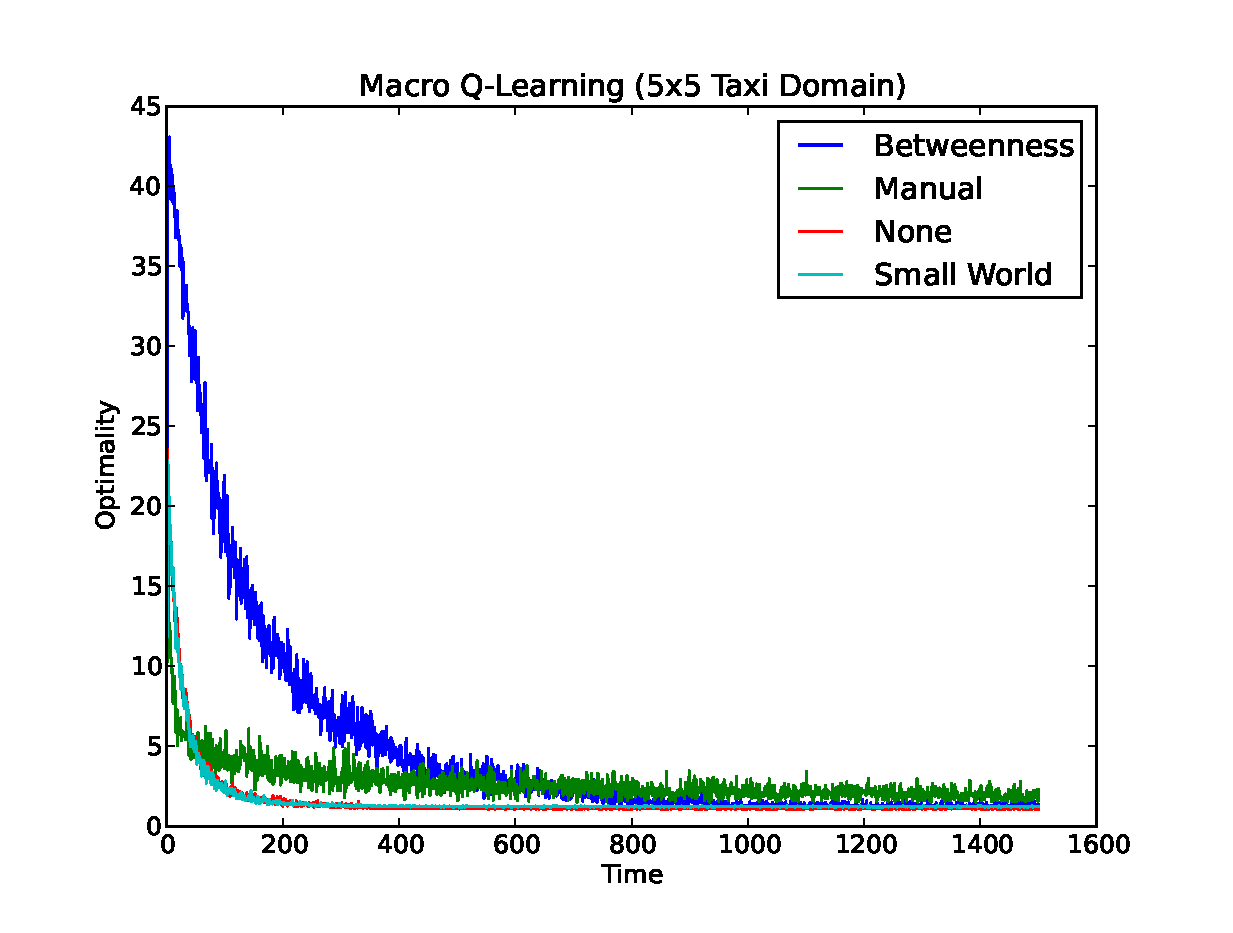
\includegraphics[width=4in]{figures/MacroQ-0_99-taxi1}
    }
    \subfigure[]{
    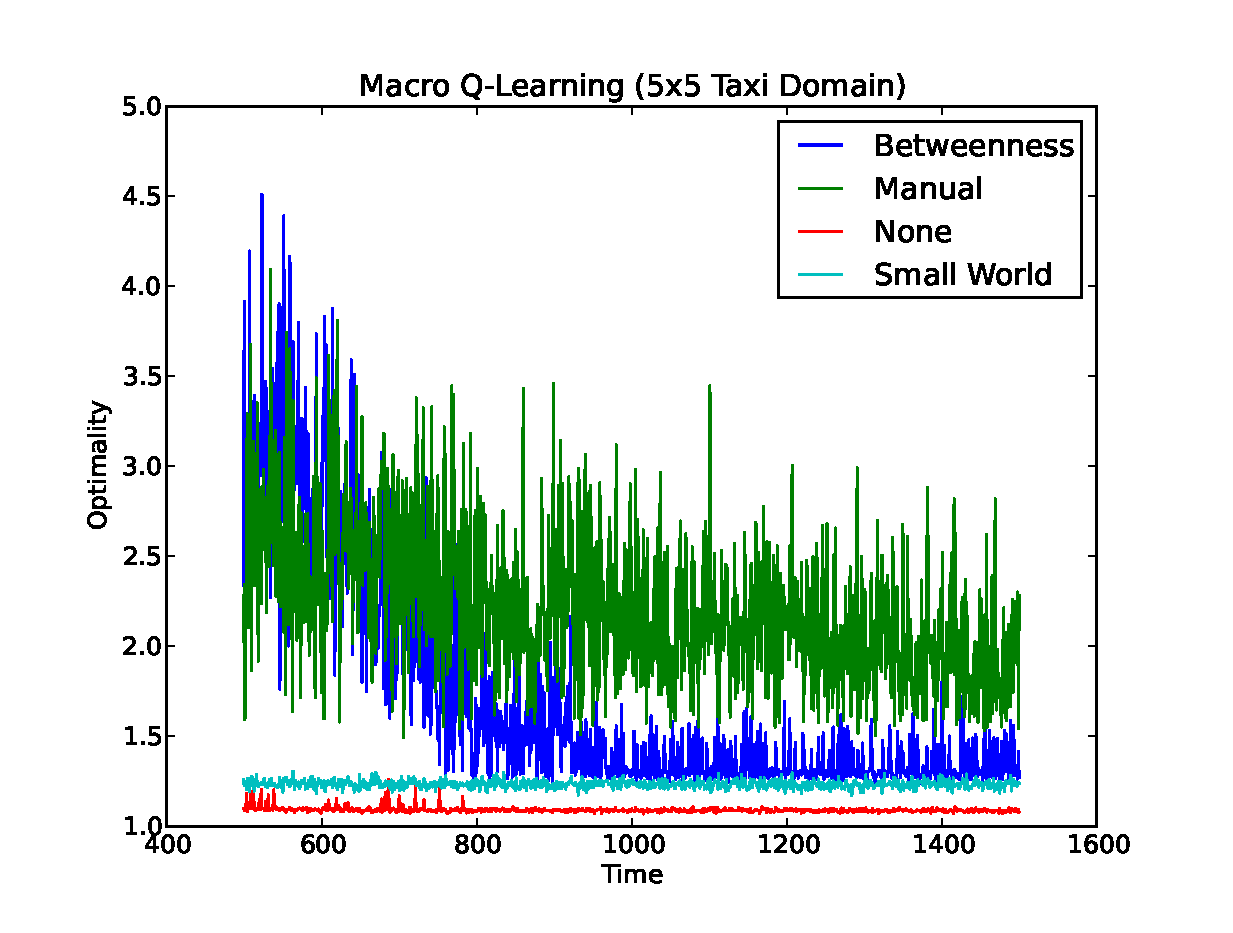
\includegraphics[width=4in]{figures/MacroQ-0_99e-taxi1}
    }
    \caption{Macro Q-learning using 20 options }
    \label{fig:MacroQ-0.99}
\end{figure}

\begin{figure}[ht]
    \centering
    \subfigure[]{
    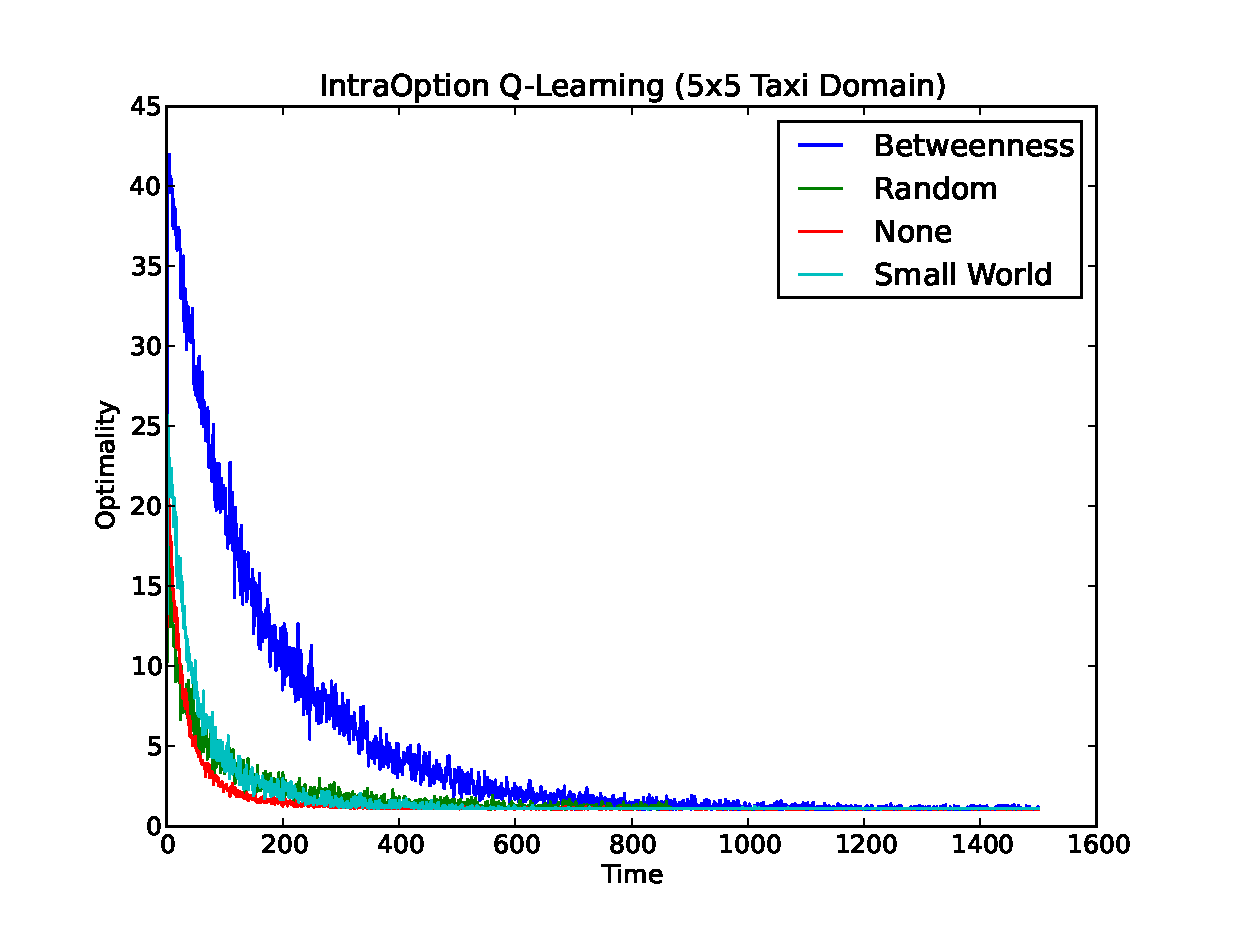
\includegraphics[width=4in]{figures/IntraQm-0_99-taxi1}
    }
    \subfigure[]{
    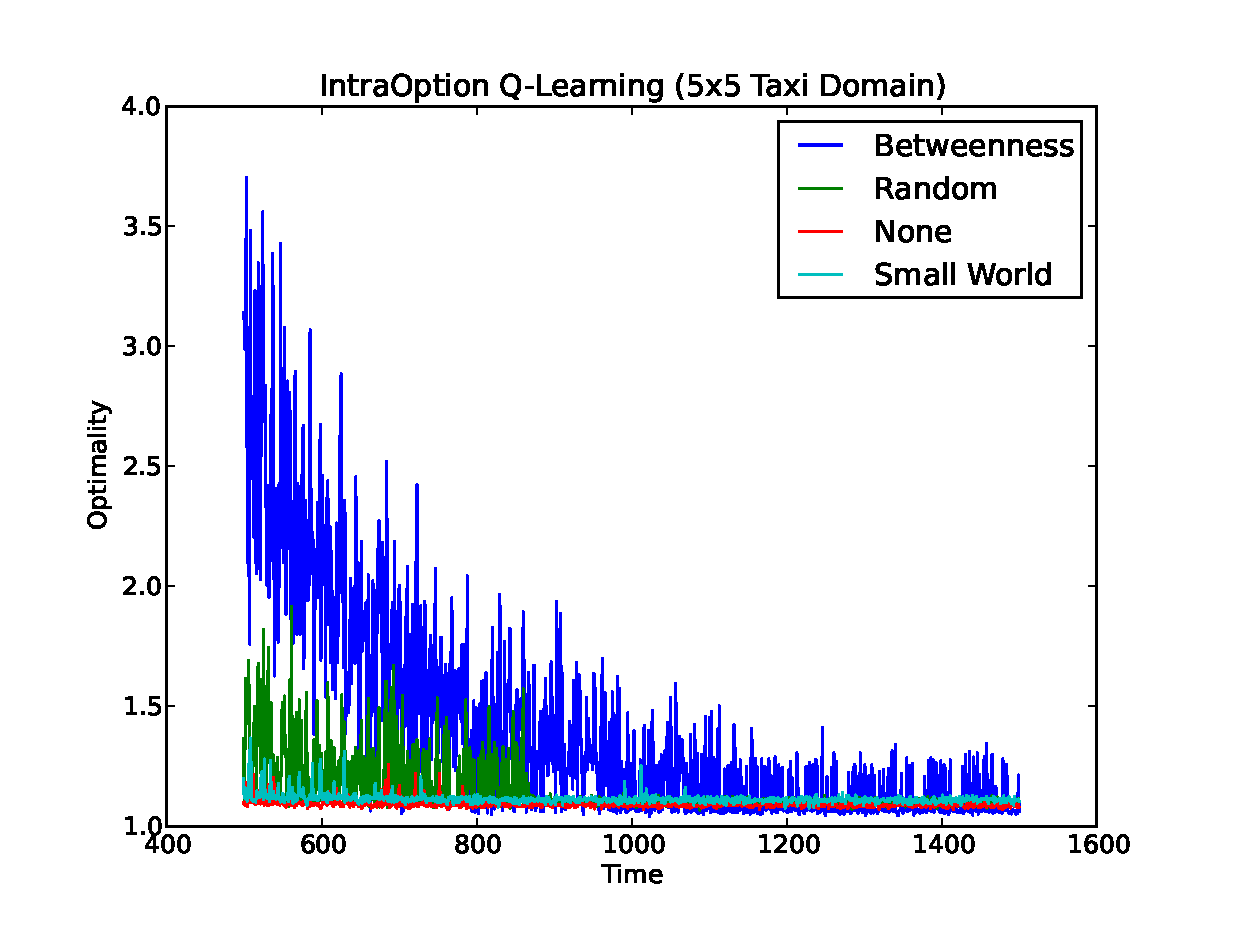
\includegraphics[width=4in]{figures/IntraQm-0_99e-taxi1}
    }
    \caption{Intra-option Q-learning using 20 options }
    \label{fig:IntraQ-0.99}
\end{figure}

\begin{figure}[ht]
    \centering
    \subfigure[]{
    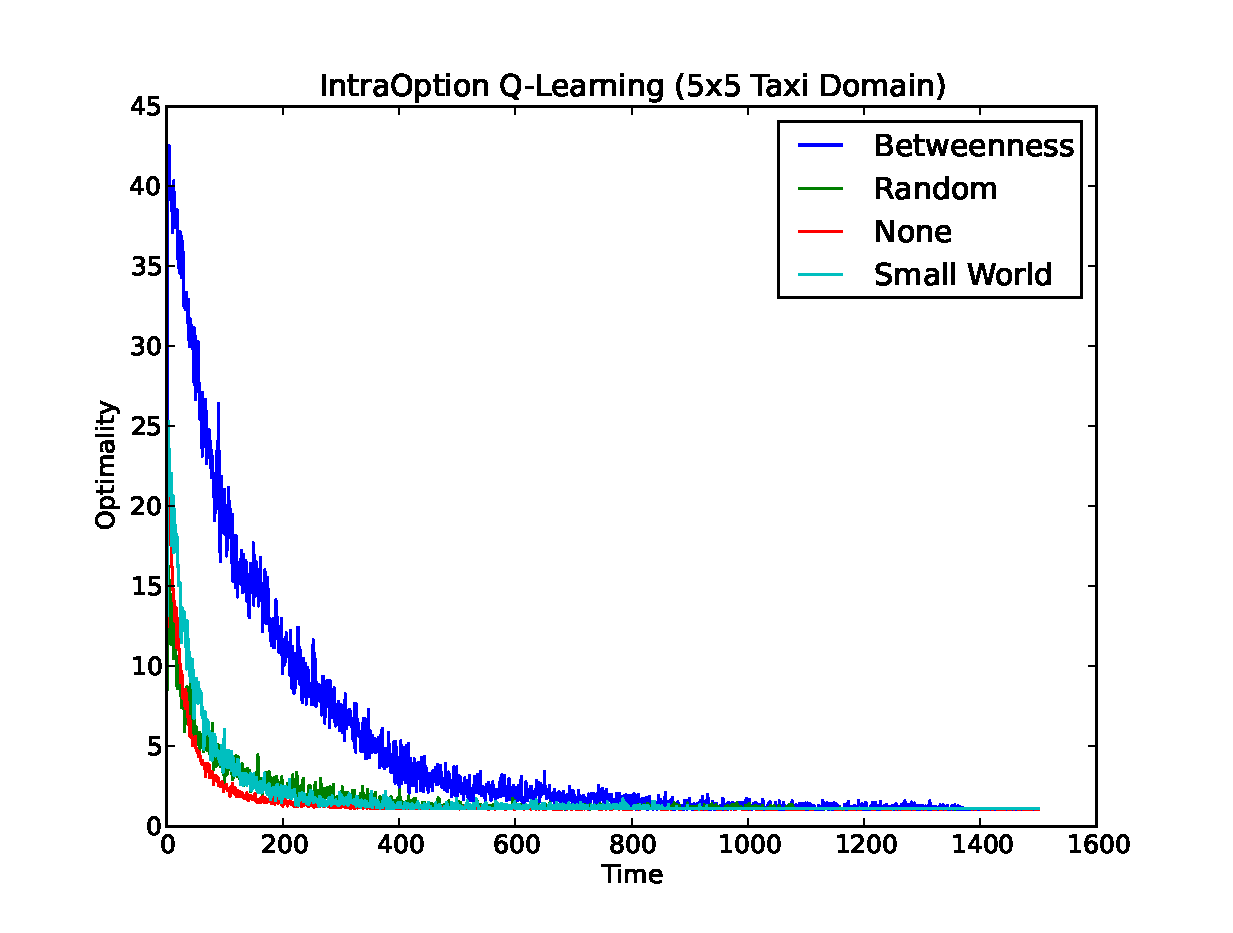
\includegraphics[width=4in]{figures/IntraQm-0_99-50-taxi1}
    }
    \subfigure[]{
    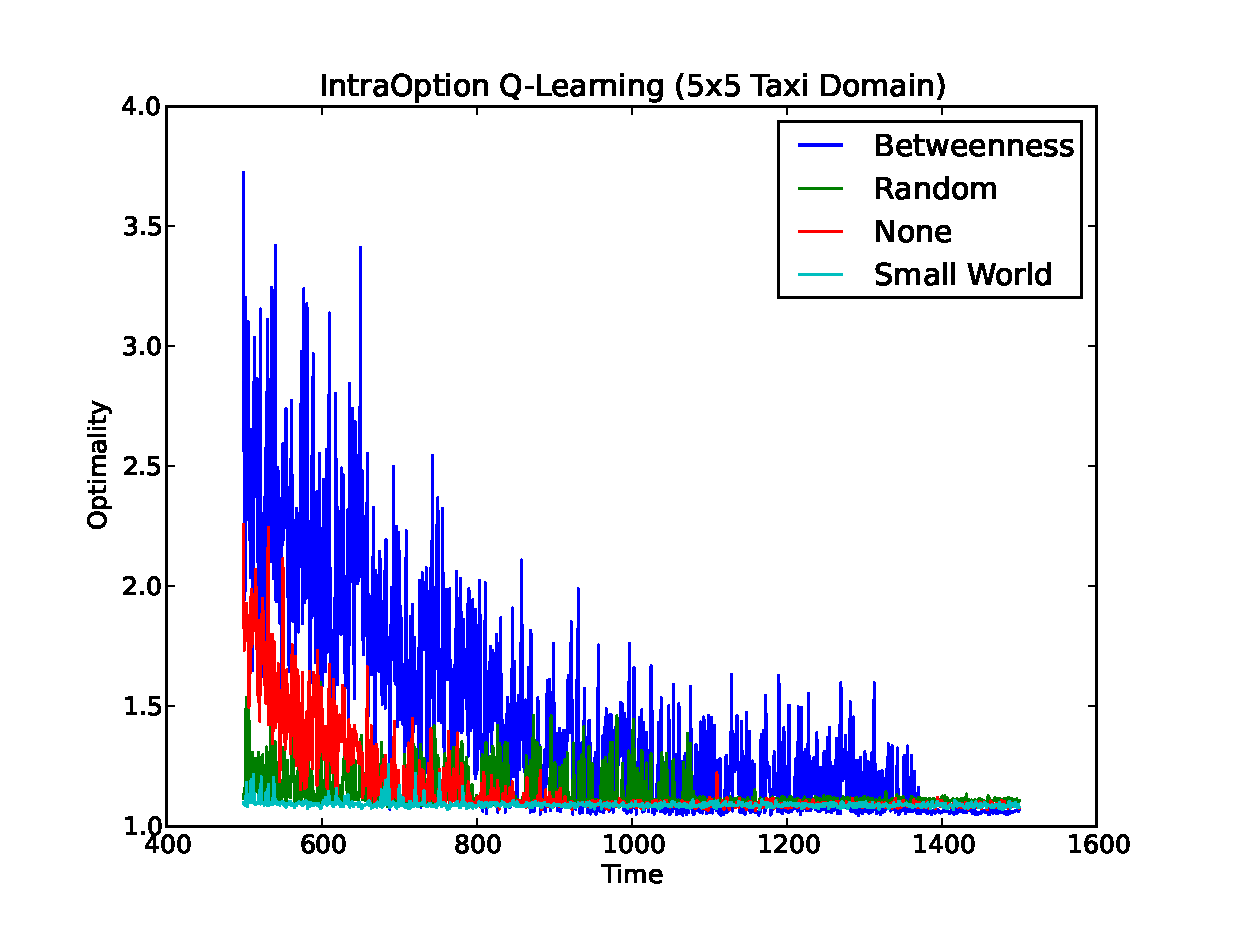
\includegraphics[width=4in]{figures/IntraQm-0_99e-50-taxi1}
    }
    \caption{Intra-option Q-learning, using 50 options }
    \label{fig:IntraQ-0.99-50}
\end{figure}

% Brief on results
We note that the agents using Small World options converge quickly to the
optimal value (i.e. 1), and have small variance. Expectedly, the performance
using Intra-option Q-learning (\autoref{fig:IntraQ-0.99}) is significantly
better than Macro Q-learning (\autoref{fig:MacroQ-0.99}). The performance of
small world options does not significantly differ between using 20 options
(\autoref{fig:IntraQ-0.99}) or 50 options (\autoref{fig:IntraQ-0.99-50}).

We find it surprising that betweenness performs worse than the remaining
schemes. Our options differ from the random options defined in \cite{Simsek} as
we select random paths instead of random nodes to which all other nodes are
connected. As a result, for many nodes there are few if any options. As adding
options also increases the number of actions that an agent can choose from, this
might have lead to the better performance of Random and Small World, which are
both path-based options.

% \begin{table}[ht]
%     \centering
%     \begin{tabular}{ r | r }
%           &  \\ \hline
%           &  \\
%     \end{tabular} 
%     \caption{ }
%     \label{tbl:rtt-summary}
% \end{table}

% \begin{figure}[s]
%     \centering
%     \includegraphics[width=5in]{filename}
%     \caption{ }
%     \label{fig:high-variance-rtt}
% \end{figure}



\bibliographystyle{amsalpha}
\bibliography{ewrl}{}

%\newpage
%\appendix

%
\section{Code}
\label{sec:code}
% \lstset{language=TCL, basicstyle=\small, showstringspaces=false, numbers=left, numberstyle=\tiny }
% \lstinputlisting{many2one.tcl}


\end{document}

